\chapter{GTFS}
\label{app:gtfs}

\Gls{gtfs} \citep{GoogleDevelopers_2006} describes the way in which transit data should be organised. There are many \emph{dataset files} specified on the \gls{gtfs} website,\footnote{\url{https://developers.google.com/transit/gtfs/reference}} each of which can be thought of as a table in a relational database. Here, I describe the tables used throughout this thesis, and even within each table I only cover relevant \emph{fields} (or columns in a database).

Each table consists of an ID columns, which corresponds to a \emph{primary key} in a relationship database. This field must be unique for each entry. Some tables also include \emph{reference IDs} or \emph{foreign keys} which point to entries in another table. For example, each entry in the \tbl{trips} table has a reference to an entry in the \tbl{routes} table. Since there can be one or more trips per route, this is considered a \emph{many-to-one} relationship in database terminology. \Cref{fig:gtfs_tables} demonstrates the relationships between the tables in \gls{gtfs}, including the essential fields in each, which are described in the following paragraphs. The quoted descriptions are taken from the \gls{gtfs} website. Note that these are only some of the fields available under \gls{gtfs}, which is continually expanding to provide more flexibility for transit providers.

\begin{figure}[tb]
  \centering
  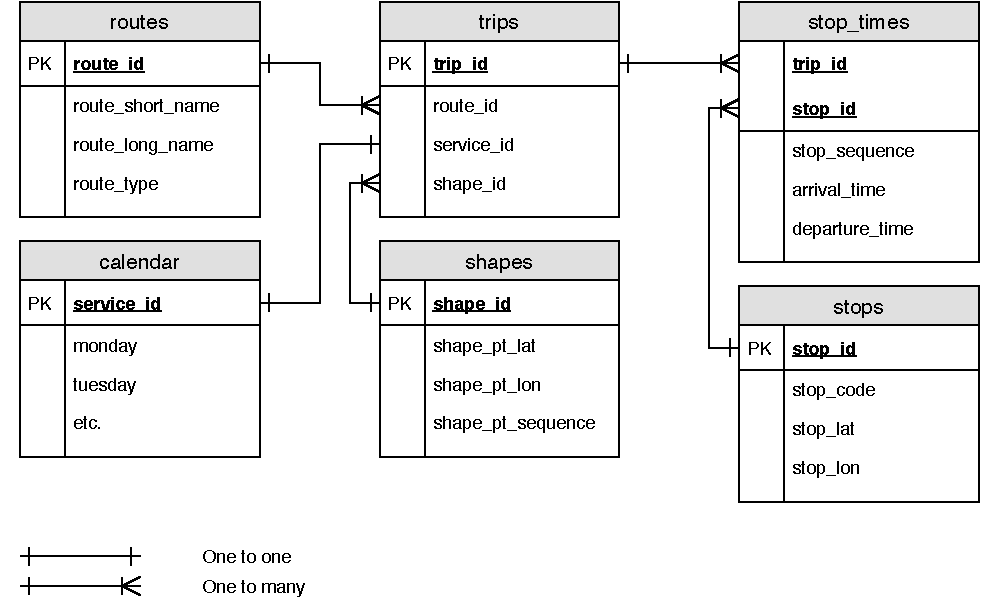
\includegraphics[width=0.9\textwidth]{figure/app_gtfs_diagram.pdf}
  \caption[GTFS diagram]{\gls{gtfs} diagram.}
  \label{fig:gtfs_tables}
\end{figure}

\subsection*{Routes}
The \tbl{routes} table contains information about individual \emph{transit routes}, ``a group of trips that are displayed to riders as a single service.''.
\begin{description}
  \item[route\_short\_name]
    generally a number (``110''), a short descriptive word (``OUTER''), or an alphanumeric sequence riders can easily identify (``NX1'').

  \item[route\_long\_name]
    describes the route in more detail, usually consisting of the destination and some major points of interest along the way: ``Ellerslie To Britomart'' or ``Three Kings To Britomart Via Mt Eden Rd''.

  \item[route\_type]
    specifies the vehicle type used for the route. For example, 2 is used for trains and 3 is used for buses.
\end{description}


\subsection*{Trips}
The \tbl{trips} table describes individual instances of routes: ``A trip is a sequence of two or more stops that occur during a specific time period.''.
\begin{description}
  \item[route\_id] references the route the trip belongs to.
  \item[service\_id] services specify on what days trips run (see Calendar table).
  \item[shape\_id] references the shape that describes the vehicle's path.
\end{description}

\subsection*{Calendar}
The \tbl{calendar} table contains ``Service dates specified using a weekly schedule with start and end dates.''. This means trips can be repeated on multiple days, which is usually divided into \emph{weekday}, \emph{Saturday}, and \emph{Sunday and public holidays} schedules. Each entry has a column for each day of the week that is either 1 if the trip runs on that day, or 0 otherwise.

\subsection*{Shapes}
The \tbl{shapes} table consists of ``Rules for mapping vehicle travel paths'', which are essentially lines on a map.
\begin{description}
  \item[shape\_pt\_lat, shape\_pt\_lon] the latitude and longitude coordinates of each point.
  \item[shape\_pt\_sequence] specifies the order of shape points for each shape.
\end{description}

\subsection*{Stops}
The \tbl{stops} table describes ``Stops where vehicles pick up or drop off riders.'', and are an essential component of our transit network used in \cref{cha:vehicle_model}.
\begin{description}
  \item[stop\_code] At least in Auckland, all stops have a unique code printed on the sign, which helps riders find them (particularly at stations where there might be multiple stops servicing different trips).
  \item[stop\_lat, stop\_lon] The physical latitude and longitude coordinates of the stop.
\end{description}

\subsection*{Stop times}
The \tbl{stop times} table consists of \emph{trip-stop} pairs, and is by far the longest table. There is one row for each stop along each trip, providing the ``Times that a vehicle arrives at and departs from stops''. Most importantly, this is the information used by the ``schedule-delay'' method currently used by Auckland Transport to predict bus arrival times.
\begin{description}
  \item[trip\_id, stop\_id] This table does not include its own unique ID, so instead unique rows are identified by unique pairs of trip and stop IDs.
  \item[stop\_sequence] defines the order of stops along a trip.
  \item[arrival\_time, departure\_time] specifies the scheduled arrival and departures times at stops. At least in Auckland, these are the same unless the stop is a \emph{layover} (the bus will, in theory, wait until the scheduled departure time). In this case, the arrival time will be earlier than the departure time.
\end{description}
